% Preamble
\documentclass[11pt]{article}

% Packages
\usepackage{amsmath}
\usepackage{graphicx}

% Document
\begin{document}
    \section{Structure from Motion Revisited}
    Structure from Motion is the task of calculating the 3D structure of a scene and the pose of cameras from
    images captured in multiple views or video frames. SfM is an important tool in many applications like
    Visual SLAM, 3D scanning, and Autonomous Driving. There are several algorithms used in SFM that help
    in reconstructing the 3D structure. In this chapter, Incremental Structure from Motion, \cite{7780814}, will be explained
    as it is the base algorithm for most papers in these criteria.

    \begin{figure}
    \caption{Structure from Motion Revistied}
    \centering
    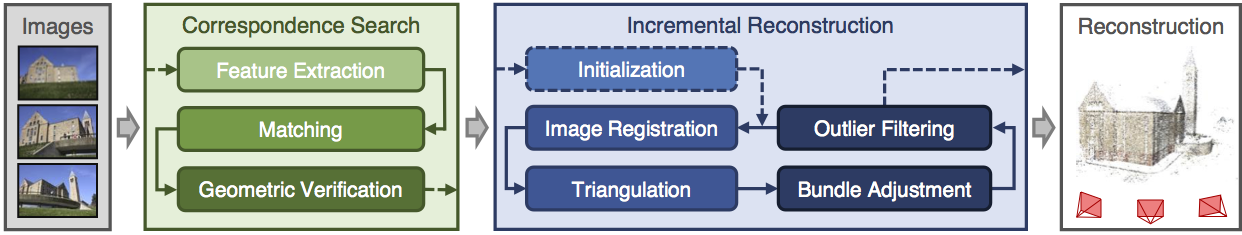
\includegraphics[width=\textwidth,height=\textheight,keepaspectratio]{images/sfm.png}
    \end{figure}

    The algorithm can be viewed as a pipeline that contains the following separated steps:

    \begin{enumerate}
        \item \textbf{Feature detection and matching:} The first step in SFM is feature detection and matching, where
        the algorithm identifies common features or points in the 2D images or video frames. These features
        can be edges, corners, blobs, or other distinctive patterns that can be detected consistently across
        the images. The algorithm, then, matches these features between different input frames. This step is one
        of the most challenging parts in SfM. Occlusion, illumination changes, perspective transformation, and moving objects
        are some of them. However, since this is a core task in many Computer Vision tasks, there has been
        tons of researches in feature detection and matching, including deep based approaches. SIFT, SuperPoint,
        S2-Net, R2D2 are often used among SfM related papers.

        \item \textbf{Geometric Verification:} raw matches are not enough for the scene reconstruction.
        Matches in similar repeated patterns, multiple objects in one image, etc, are some issues that may cause wrong
        poses and 3D points. Outliers must be removed from the list of matches. Therefore, by using RANSAC and epipolar
        geometry, camera matrices, i.e. homography(H), Essential(E), and Fundamental(F) matrices, can be calculated
        to verify the geometric consistency of the reconstructed 3D points and camera poses.
        Without geometric verification, the reconstructed 3D model may contain errors that can lead to incorrect result.

        \item \textbf{Reconstruction Initialization:} If the pipeline is considered as an iterative or sequential process,
        a starting point is essential. Choosing a good initial pair of images is, also, so important. At the end of
        each iteration, the camera parameters and 3D structure are optimized, i.e. the differences between
        the observed 2D features and the projected 3D points are minimized. Without a good initial estimate,
        the optimization process usually doesn't converge and stuck in local minima. A good initial pair can be
        chosen from the top of list of images that are sorted based on the number of correspondences matches.

        \item \textbf{Image Registration and Triangulation:} After initialization, the algorithm uses triangulation to estimate
        the 3D position of the matched features in every new image. Triangulation involves finding the intersection point
        of two or more rays of light that originate from the camera and pass through the 2D features. The intersection
        point represents the 3D position of the feature in the scene.

        \item \textbf{Bundle Adjustment:} As the previous processes involve some errors, there may be inconsistencies
        or misalignment between the estimated camera parameters and the triangulated 3D points, and it could get worse
        and worse for every new image. Bundle adjustment refines those parameters by rewriting the non-linear
        reprojection equations which contain camera poses' matrices, calibration parameters, and, 3D points positions.
        It typically uses an optimization algorithm such as Levenberg-Marquardt to minimize
        the reprojection error. The optimization problem can be non-linear and high-dimensional, and it may take a
        long time to converge to a good solution. However, bundle adjustment can significantly improve the accuracy
        of the reconstructed 3D scene and camera poses.

    \end{enumerate}

    \newpage
    \section{Related Works}
    Structure of Motion is a core task for many projects. It gives the ability to obtain detailed 3D models
    of the environment from 2D images or video sequences. This information can be used widely in many other
    low level tasks like object tracking, object detection, and also, understanding the scene and detecting speed and
    positions of objects for autonomous driving as a high level tasks. Therefore, the accuracy and the speed
    of the algorithm is crucial. As an example for accuracy, a tiny error, e.g. 1 degree, in the rotation of
    a camera could cause several meters misalignment in the coordinates of the points especially in open scenes.
    Therefore, over the past few decades, there has been lots of efforts to improve each part of these algorithms.
    Here is a review of the recent best papers in this area:

    \newpage
    \subsection{Researches in Feature Matching}
    Each paper usually focuses on one or two tasks in the SfM pipeline. The first step, feature matching,
    is one of core tasks in many Computer Vision applications as they are used to identify the corresponding
    matches among the input images. Some of the chanllenges are deformation in different viewpoints, occlusion,
    illumination changes, moving objects, etc. Because of that, there has been tons of reasearches in this area.

    \paragraph{~\cite{Dusmanu2020Multi}} tracks each keypoint in all input images, and creates a tentative
    matches graph with keypoints as nodes and matches as edges. Each keypoint is known by its surrounding pixels
    information. So, a h*w patch is selected around the feature and a d dimensional descriptor id calculated by
    a neural network with Siamese architecture. Then, for each pixel, a dot product similarity is caluclulated
    with every pixel in the other patch (h*w*h*w dimension). After normalization, a translation vector ($T_{u->v}$)
    is obtained which refines the position of keypoint by using a correlation layer as regression. Next, as each
    keypoint could be seen in multiple images,
    a single incorrect match or displacement can cause cascade of errors in the results. Therefore, another
    refinement is also applied to the track of each keypoint detected in multiple images. For each track,
    a non-linear equation for minimizing dot similarity between patches is optimized. The idea of this paper
    is also used in \cite{lindenberger2021pixsfm} which will be described in detail in the next chapter.

    \begin{figure}
    \caption{Paper: Multi-View Optimization of Local Feature Geometry}
    \centering
    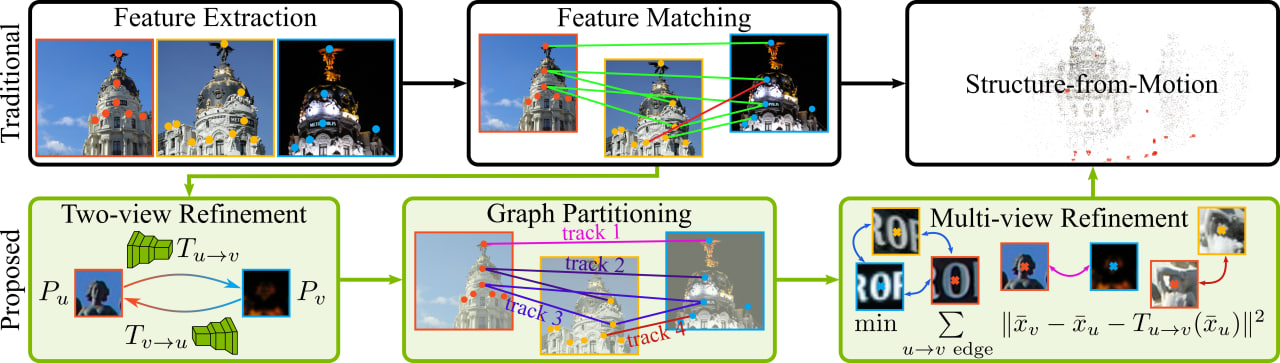
\includegraphics[width=\textwidth,height=\textheight,keepaspectratio]{images/dusmano.jpg}
    \end{figure}

    \paragraph{~\cite{wang2021deep}} uses optical flow to predict dense correspondences between two frames. The method is
    able to find more and better matching points and therefore more accurate poses and depth maps, especially for
    textureless and occluded areas. They use DICLFlow, explained in \cite{wang2020displacement} to generate
    dense matching points between two consecutive frames. \cite{wang2020displacement} uses a displacement invariant matching
    cost learning strategy and a soft-argmin projection layer to ensure that the network learns dense matching
    points rather than image-flow regression. Noisiy matches like moving
    objects are filtered out by the means of SIFT features. After calclulating the essential matrix , using
    the classic five-point algorithm with RANSAC scheme, and the dense matching points from optical flow estimation,
    the dense depth map is computed by performing triangulation. Before this process, the matching is performed
    again by constraining the search space to epipolar lines computed from the relative camera poses. They filtered
    out noisy matches twice which means dense matches by optical flow are too noisy. High number of matches is good
    for obtaining more points in sparse reconstruction. However, they tend to be noisy. They also,
    introduced a Scale-Invariant Depth Module to deal with the up-to-scale relative pose and mismatch between the
    scale of the camera motion and the scale of the depth map. Up to scale problem means that while the
    relative positions of the reconstructed points are accurate, their absolute positions in the real world
    are not known unless there is additional information, such as the size of an object in the scene or the
    distance between two known points. In order to deal with this problem, this paper generates a number of matching
    candidates with different depths with the same distance. And thn, a plane-sweep powered network minimize
    the loss function which is the position displacement of the features in the flow.

    \begin{figure}
    \caption{Paper: Deep Two-View Structure-from-Motion Revisited}
    \centering
    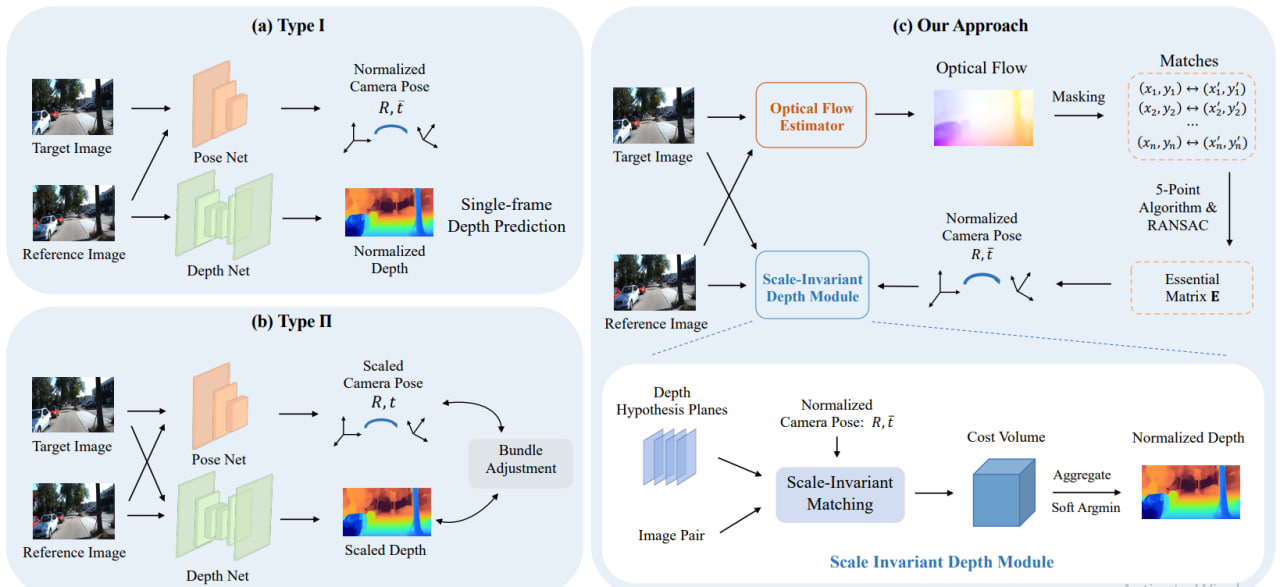
\includegraphics[width=\textwidth,height=\textheight,keepaspectratio]{images/deep_two_sfm.jpg}
    \end{figure}

    \paragraph{} There are more researches in feature matching step, \cite{revaud2019r2d2} introduced a deep based feature
    detector that is trained with self-supervision, and simultaneously outputs sparse, repeatable and reliable
    keypoints that outperforms handcrafted detectors and descriptor.
    \cite{dusmanu2019d2net} is another deep based approach to feature matching that showed great performance.
    \cite{detone2018superpoint} is a self-supervised framework that can adapt itself to homography challenges
    and multi-scale problems.

    \newpage
    \subsection{Researches in Bundle Adjustment}
    Bundle Adjustment algorithms optimizes the camera parameters and the output points by minimizing the
    difference between the observed image points and the corresponding projected 3D points. However, there
    are some disadvantages with this technique. Bundle Adjustment requires solving a large system of
    non-linear equations, which can be computationally expensive, especially for large datasets. This can be a
    significant drawback, especially when processing real-time data. It can be sensitive to the initial values.
    If the initial values are not accurate, the optimization may fail to converge. The optimization problem can have
    many local minima which means high probability in resulting in suboptimal or incorrect results. Also, inaccurate
    optimization can increase the error exponentially in the subsequent iterations. In the next chapter, it will be
    shown that the most time-consuming part in Structure from Motion is this step.

    ~\cite{tang2019banet} mainly focuses on bundle adjustment step in SfM pipeline. They implemented feature-metric
    bundle adjustment that minimizes feature-metric errors between feature pyramid of images obtained by CNNs.
    As \cite{LSDSLAM} says, there are two types of BAs:
    - Typical geometric BA with re-projection error(pixel coordinates): Only a few pixels, i.e. keypoints, are
    taken into account which comes with keypoints detection and matching challenges
    - Photometric BA algorithm(all aligned pixel, pixel intensities as error): It has good accuracy,
    especially at less textured scenes. However, the disadvantages would be sensitivity to camera exposure,
    illumination changes, and outliers such as moving objects. Also, considering all pixels would increase
    the computation dramatically.
    BA-Net creates a pyramid of features for each image and align them. The featire pyramid is generated by
    multi-scale hierarchy of CNN(DRM-54, \cite{yu2017dilated}) to construct feature pyramids. Then, the BA equation
    to minimize would be:
    \[ e^f_{i,j}(X) &= F_{i}(\pi(T_{i},d_{j} \cdot q_{j}))-F_{1}(q_{j}) \]
    where $F = {F_{i} | i = 1 to N_{i}}$ are the feature pyramids of images $I = {I_{i} | i = 1 to N_{i}}$.

    For the generation of dense reconstruction, the depth of all pixels in all images are required. However, the
    computation of these values is super expensive. This paper, also, uses a great approach to deal with this
    issue that is mentioned in \cite{tateno2017cnnslam} and \cite{yang2018deep}. A set of arbitrary basis depth maps
    is created. Then, the final depth map is generated as a linear combination of these basis depth maps:
    \[ D = ReLU(w^T * B) \]
    "w" will be optimized in our BA-Layer. Generally, this idea is great when the number of
    values to calculate is too high.

    They are many papers that tackle Structure from Motion problems under Visual SLAM (visual simultaneous
    localization and mapping) and odometry subjects.
    DROIDSLAM \cite{teed2022droidslam} use neural networks to estimate dense flow fields which are subsequently
    used to optimize depth and camera pose. For each new video frame, DROID-SLAM produces a differentiable Dense
    Bundle Adjustment and Gauss-Newton solver to update camera poses and dense per-pixel depth to maximize their
    compatibility with the current estimate of optical flow. \cite{teed2022deep} utilizes a neural network to
    generates a collection of patches from incoming frames. They update the differentiable bundle adjustment layer
    by tracking patches' trajectory using A recurrent neural network. They demonstrate that their end-to-end system
    causes strong generalization on real video, patch-based correspondence improves efficiency and robustness over
    dense flow, and using RNNs allow end-to-end learning of reliable feature matching.

    \newpage
    \subsection{Pixel-Perfect Structure-from-Motion with Featuremetric Refinement}
    Among all reviewed paper, \cite{lindenberger2021pixsfm} has the best performance. The paper
    proposes two stages to improve the accuracy of structure-from-motion for 3D reconstruction.
    In the first stage, the initial keypoint locations are adjusted prior to any geometric estimation
    by optimizing a direct cost over dense feature maps. In the second stage, 3D points and camera poses
    are refined using a featuremetric error based on dense features map obtained by Convolutional Neural Network.
    The paper produced accurate reconstructions and scaled well to large scenes with thousands of images.
    Also, their contribution could be used as an extra step in the SfM pipeline. So, it can be easily
    integrated with any other papers' contributions.

    \begin{figure}
    \caption{Paper: Pixel-Perfect Structure-from-Motion with Featuremetric Refinement}
    \centering
    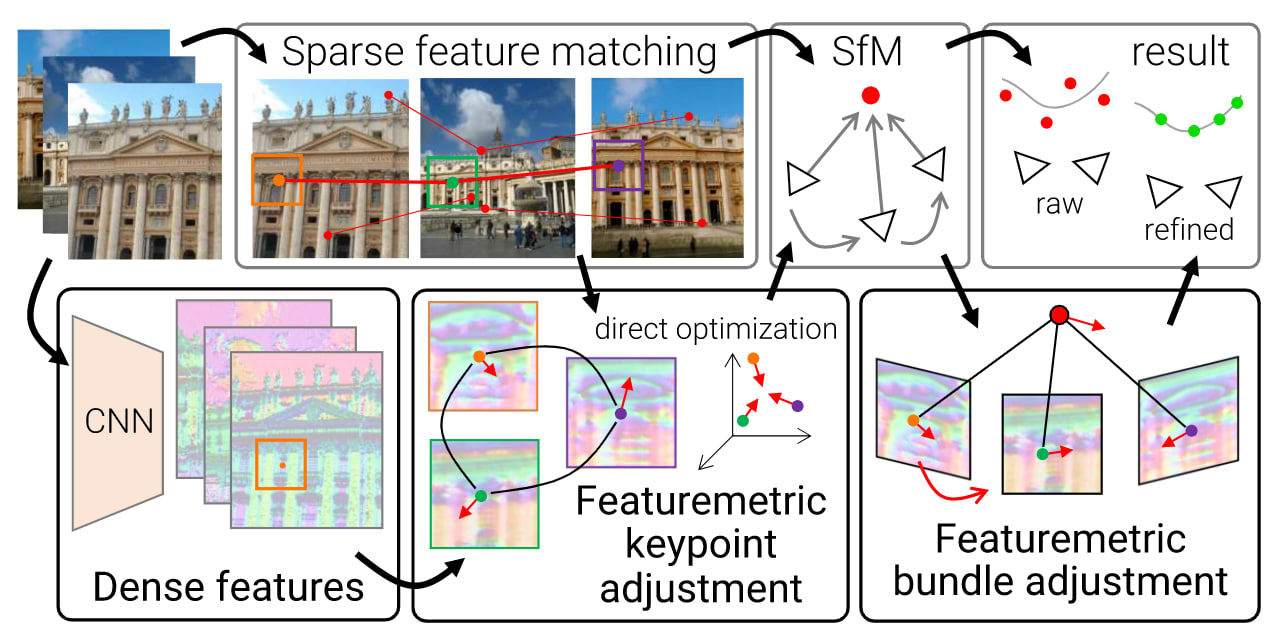
\includegraphics[width=\textwidth,height=\textheight,keepaspectratio]{images/pixel_perfect.jpg}
    \end{figure}

    They use the initial idea of \cite{Dusmanu2020Multi} that separates the tracks for each keypoint, and
    adjusts their locations by optimizing the geometric cost over the input images which the keypoint
    is seen. \cite{Dusmanu2020Multi} improved SfM, but has limited accuracy and scalability. To solve that, This paper proposes
    a feature map for each image using convolution neural networks. The feature map condenses the dense
    information from surrounding pixels into a vector for each pixel. The reason behind this step is the
    fact that refining geometry is an inherently local operation, not based solely on the pixel, and the
    dense information only needs to be locally accurate and invariant but not globally discriminative.
    For the first stage, i.e. keypoint adjustment refinement, the locations of 2D keypoints belonging to the same
    track j is refined by optimizing its featuremetric consistency along tentative matches. The loss function is

    \[ E_{FKA}^j &= \sum_{(u,v) \in M_{j}}w_{uv}\lVert F_{i(u)}[p_{u}] - F_{i(v)}[p_{v}]\rVert_{\gamma} \]

    which means the . After computing the loss value, the translation vector that refines the location of the
    keypoint is optimized with respect to a gradient descent update that considers the local image derivatives:
    # TODO


    In compare to \cite{Dusmanu2020Multi}, optimizing by the cost of feature maps instead of the patch neighboring
    pixels has better efficiency.

    In the second stage, i.e. bundle adjustment refinement, typical approach uses the euclidean distance between the point and
    its reprojected 3D from another view. However, this paper considers the difference between the feature vectors
    of the point and the feature vector of the point where the 3D point is reprojected. The loss fubnction is

    \[ E_{FBA} &= \sum_{j} \sum_{(i,u) \in \tau_{j}}\lVert F_{i}[ \prod (R_{i}P_{j} + t_{i},C_{i})] - f^j\rVert_{\gamma} \]


    Also, instead of acquiring the cost equation for each pair of views, one image is considered as a reference,
    and the cost equations are written between the reference image and the rest of views. it reduces the number
    of residuals from $O(N^2)$ to $O(N)$. This is not good for the sequential video frames. Because newer frames will be
    too far from the reference image. However, it is achievable if the new input is a batch of new images, and
    the refinement is applied to each batch separately.


    As it is mentioned earlier, this paper can be integrated with other approaches. In their experiment,
    \cite{revaud2019r2d2}, \cite{detone2018superpoint}, \cite{dusmanu2019d2net}, and \cite{detone2018superpoint}
    are used as base feature detector, and then applied refinement. In ETH3D dataset, \cite{Schops_2019_CVPR},
    it is reported that accuracy is improved with the average of 10 to 15 percent for each base feature detector.
    And, the runtime is decreased significantly in compare to \cite{Dusmanu2020Multi}.

    In order to verify that this paper can actually refine the reconstruction, a test dataset is
    created from a cereal box on a table, and dense 3D point cloud (\ref{fig:cereal}) is obtained by COLMAP (left screenshots)
    and refined by pixel perfect (right screenshots). It can be clearly seen that their approach is promising"

    \begin{figure}
    \caption{Compare Pixel Perfect refinement}
    \centering
    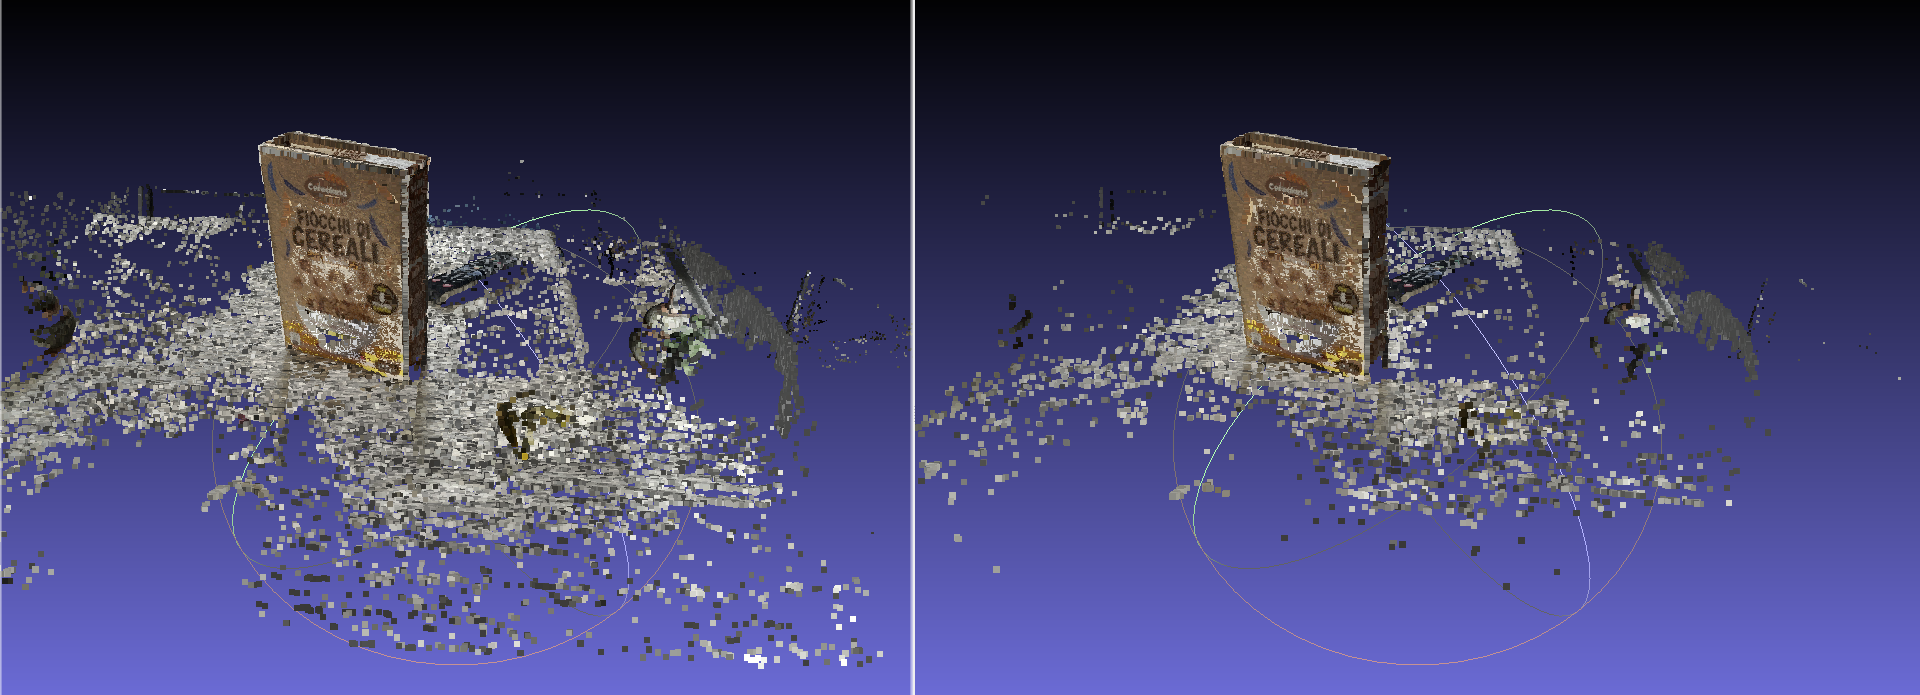
\includegraphics[width=\textwidth,height=\textheight,keepaspectratio]{images/cereal.1.png}
    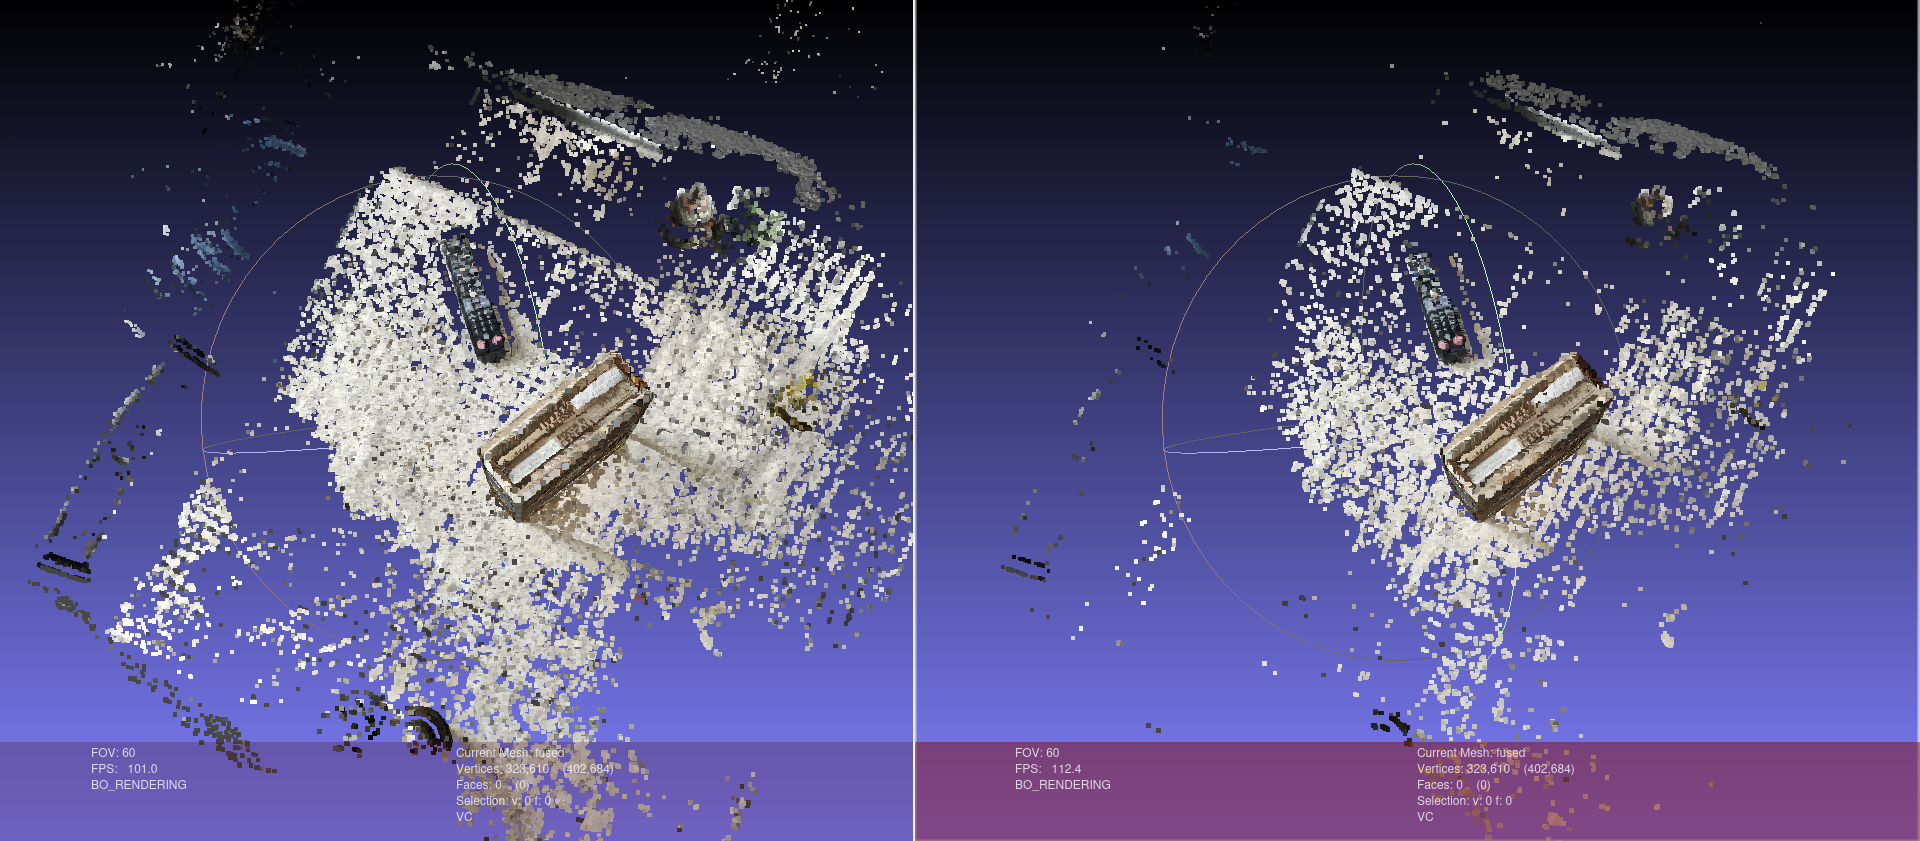
\includegraphics[width=\textwidth,height=\textheight,keepaspectratio]{images/cereal.2.png}
    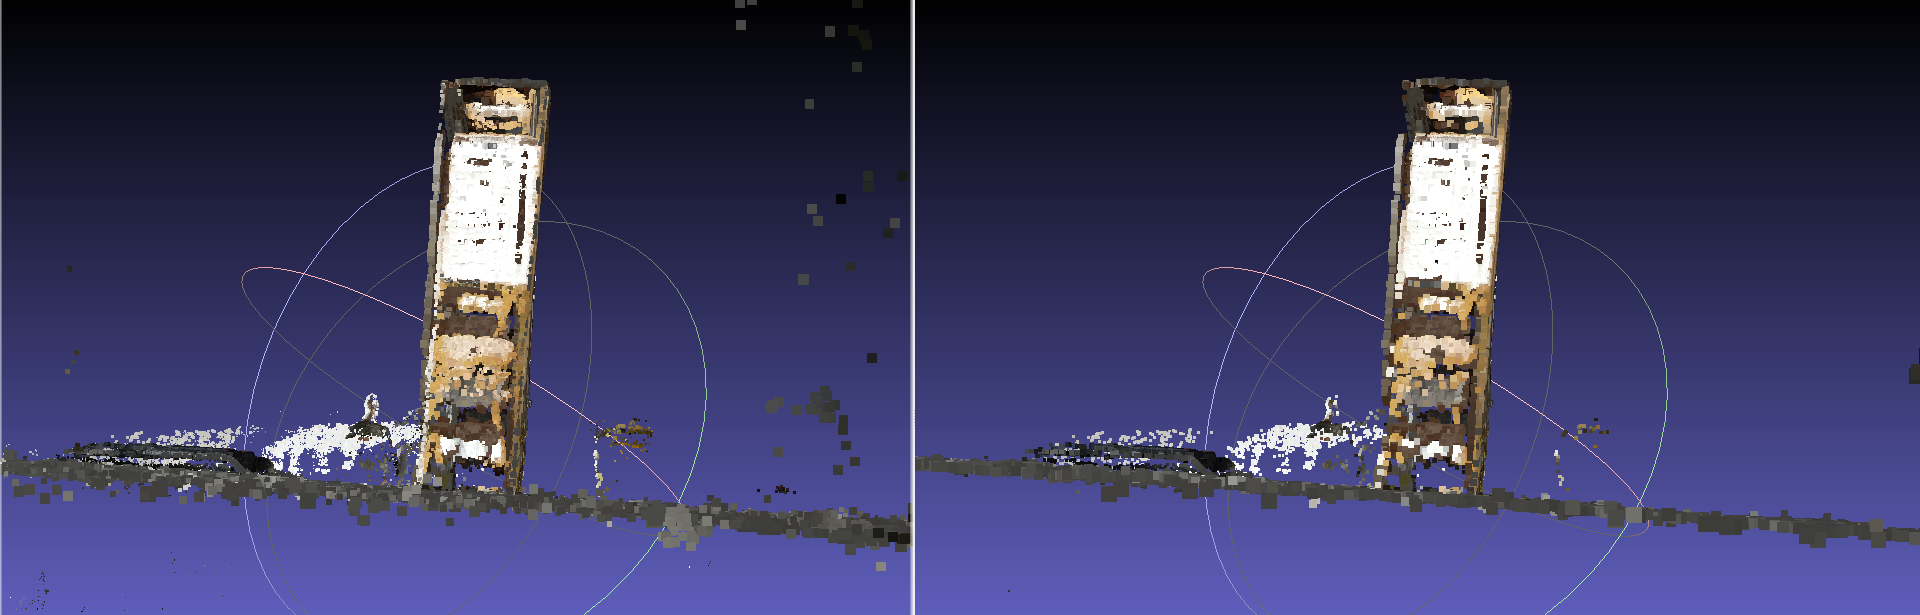
\includegraphics[width=\textwidth,height=\textheight,keepaspectratio]{images/cereal.3.png}
    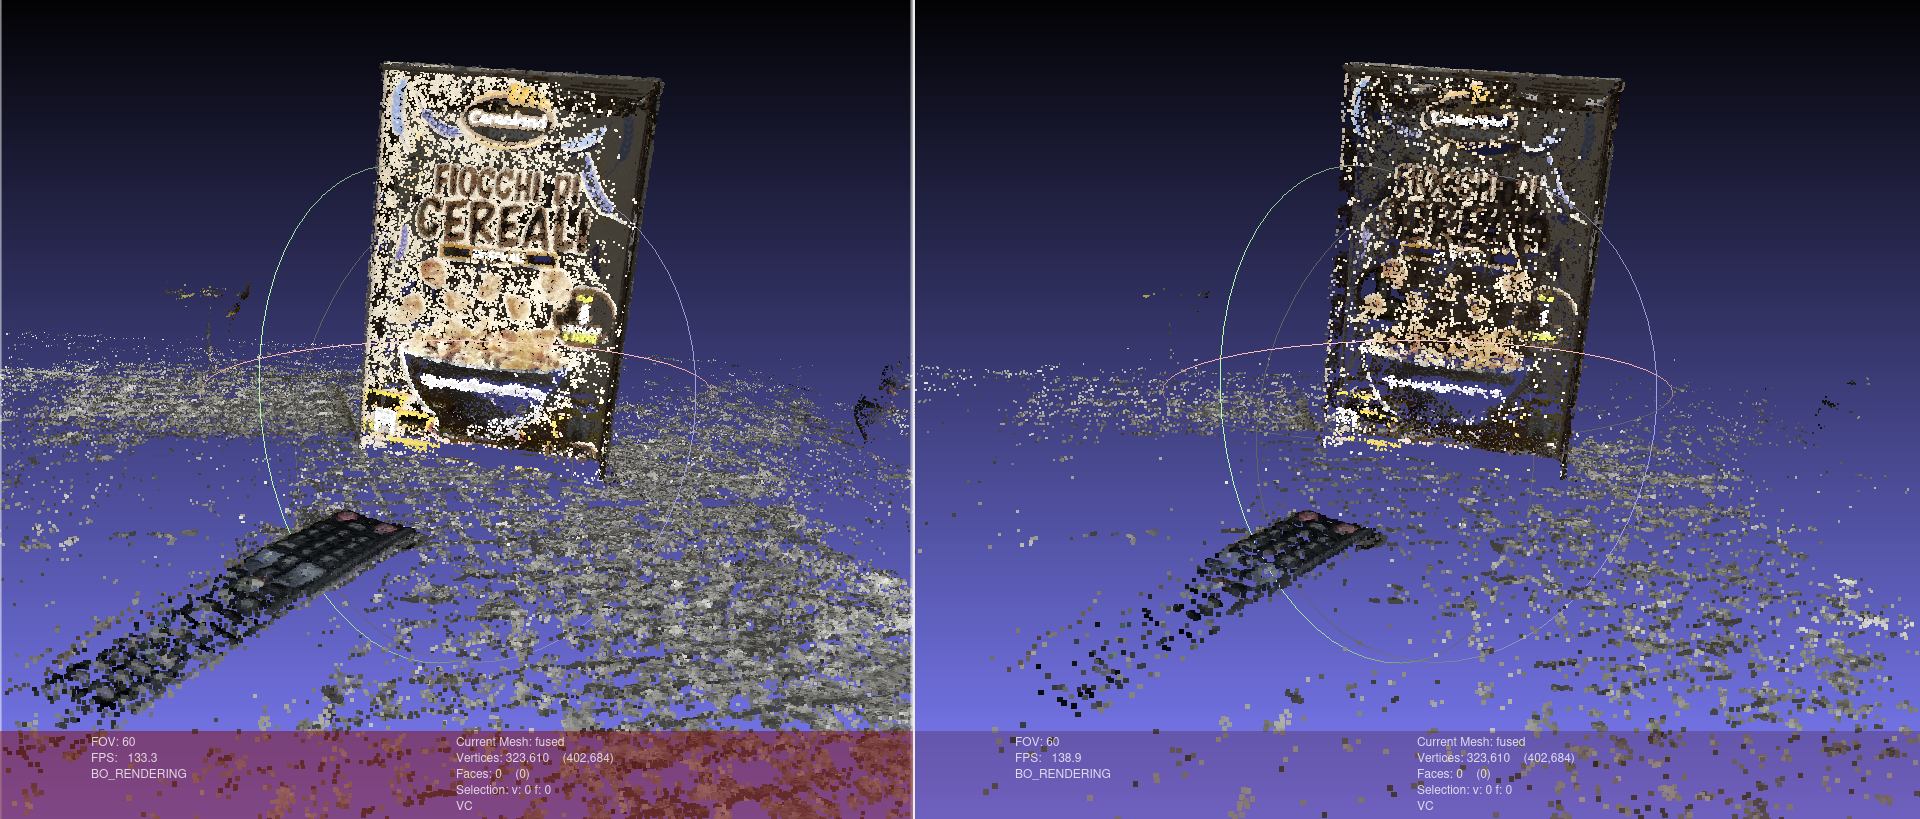
\includegraphics[width=\textwidth,height=\textheight,keepaspectratio]{images/cereal.4.png}
    \label{fig:cereal}
    \end{figure}


\end{document}
